\label{chap2}

This chapter describes the dynamic model derivation of the soft robotic manipulator. First, the soft robotic system used in this work is further detailed. Then the configuration space of the soft robot is described. Once this configuration space is determined, the forward kinematics at position and velocity level are derived. These forward kinematics allow for the derivation of the dynamic model. 


%%%%%%%%%%%%%%%%%%%%%%%%%%%%
%%%%%%%%%%%%%%%%%%%%%%%%%%%%

\section{System description}

The soft robot studied in this work is composed of a visco-elastic polymer using selective laser sintering technology. This manufacturing method is well suited to print hollow compartments, that allow for inflation. The elastomer has a low Young's modulus and is able to sustain large strains. These characteristics allow to induce large deformations with relatively low pressures. The geometry of the soft robot is best described by two bellows placed in parallel. Over the vertical axis, the bellows are connected to each other, creating the centre line of the actuator. The bellows are connected by a flanges at the top and bottom. The bellows can be inflated individually via air inlets created in the flange at one end of the actuator. The other end is closed, allowing to pressure the bellows. Since each bellow can be inflated independently, the entire actuator can increase its length and change orientation. Pressurizing both bellows equally will result in a near pure elongation of the soft robot. Creating a pressure difference will cause the soft robot's upper flange to rotate. The following assumption is made with respect to the robot's task space:

\begin{theorem}
Strains in the soft robot imposed by pneumatic actuation change the soft robot's length and orientation. Strains causing out of plane motion are deemed negligibly small, and can not be actively controlled. The soft robot's task-space therefore restricts itself to the 2 dimensional plane.
\end{theorem}

This assumption allows to describe the configuration of the soft robot in a two dimensional Cartesian plane. Since the soft robot has no clear end-effector in the form of a gripper, a point on the body is assigned to be the end-effector. This point is situated at the geometric midst of the upper flange. The lower flange with the air inlets is fixed, here its geometric midst is defined as the origin. Altering the bellow pressure can therefore change the soft robot's end-effector position. Based on above assumptions a kinematic model of the soft actuator is developed. 


\section{Cosserat beam theory}

To describe the kinematics of the soft actuator, a Cosserat beam model is used \cite{Boyer2019}. This beam model can be thought of as a continuous one-dimensional curve representing the robot's backbone. This backbone is represented in Figure (\ref{fig2:kinematicschematic}) as the black dashed curve. This curve describes the configuration of the soft robot as a function of space and time. Therefore, this function is dependent on spatial coordinate $\sigma \in \mathbb{X}$ within bounded domain $\mathbb{X} \in [0,L_0] \subset \mathbb{R}$, where $L_0$ is the nominal length of the actuator. Furthermore, a temporal coordinate $t \in \mathbb{T}$ with $\mathbb{T} \in [0,T]$ is defined. Under the assumption that the soft robot's task space is a two-dimensional plane, the rotation of any point $\sigma$ at time instance $t$ is given by rotation matrix $R(\sigma,t) \in \mathbb{SO}(2)$. Where $\mathbb{SO}(2)$ belongs to the special orthogonal group within Lie group theory. This matrix allows to express rotation of points on a two-dimensional surface, and is isomorphic to the circle group. Similarly, the position of that point is given by position vector $p(\sigma,t) \in \mathbb{R}^2$. Therefore, the Cosserat beam model creates a local frame at $\sigma$ which is tangential to this curve. This allows to describe position and rotation for any point $\sigma$ and time instance $t$ along the backbone of the soft manipulator by,


\begin{equation}
    g(\sigma,t) = \begin{pmatrix}  R(\sigma,t) & p(\sigma,t) \\ 0_3^\top & 1 \end{pmatrix} \in \mathbb{SE}(2),
    \label{eq2:g}
\end{equation}

where $\mathbb{SE}(2)$ is the Euclidean group within Lie algebra of rigid body transformations in $\mathbb{R}^2$ \cite{Sola2018}. In order to derive forward kinematics another assumption has to be made with respect to this backbone curve $g(\sigma,t)$.

\begin{theorem}
Curve  $g(\sigma,t)$ is a continuous differential function $ \forall t \in 
\mathbb{T} $ and $\forall \sigma \in \mathbb{X}$
\end{theorem}

This assumption demands that derivatives of the backbone with respect to time and space are also continuous. These derivatives are essential in determining the strain and velocity field of the soft robot actuator. This strain field allows to determine the time-invariant forward kinematics. Whilst the velocity field will be used in determining the system dynamics. First we try to solve the forward kinematic problem by computing the strain field.

\newpage

\begin{figure}[H]
    \centering
    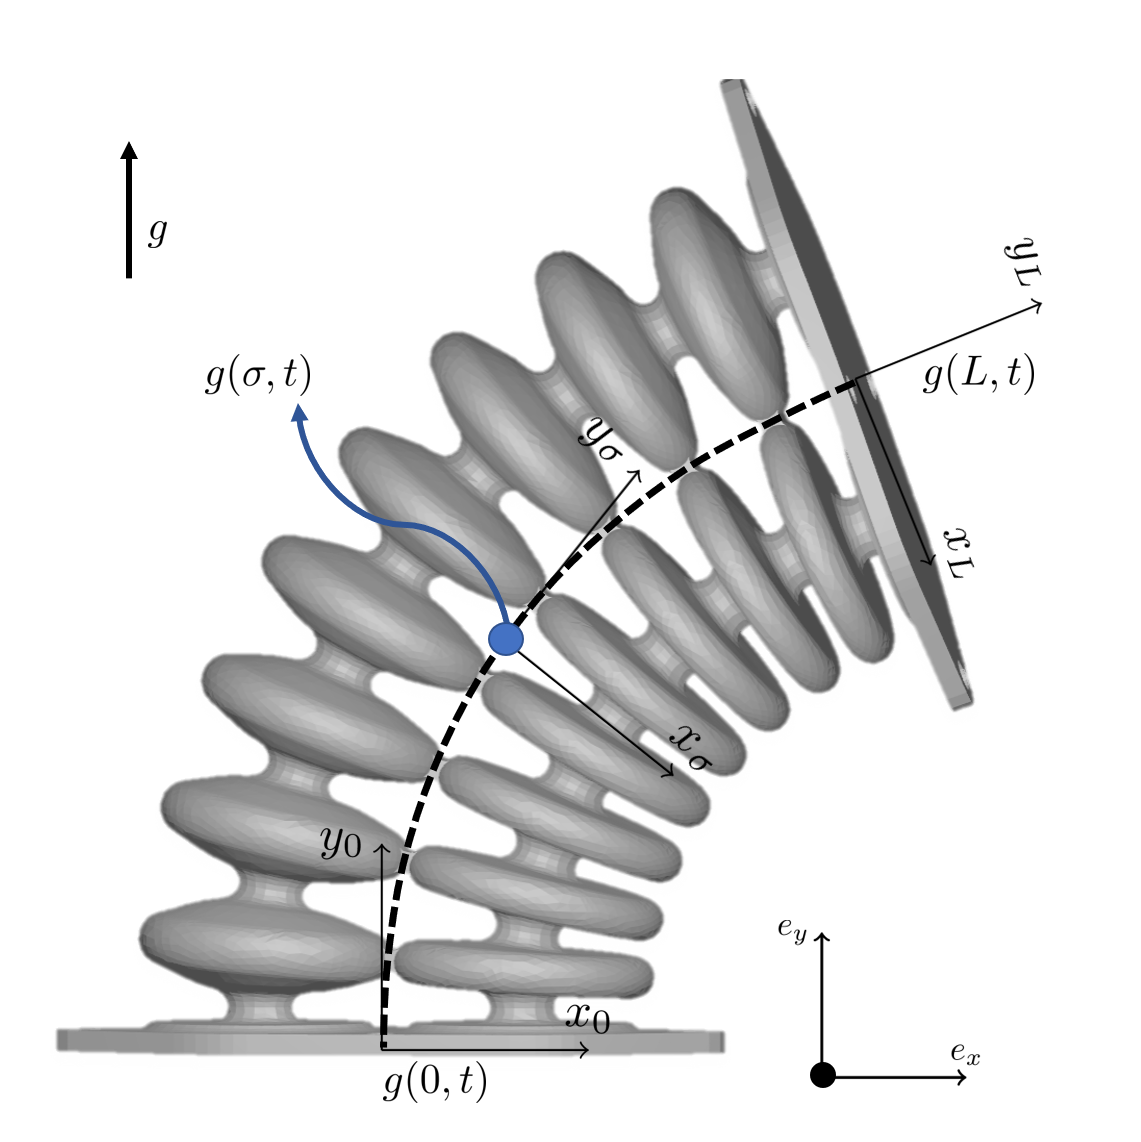
\includegraphics[width=0.55\textwidth]{Figures/Chapter2/actuatorschematic.png}
    \caption{Planar soft actuator with the backbone curve $g(\sigma,t)$.}
    \label{fig2:kinematicschematic}
\end{figure}

\section{Computation of the strain field}

The strain field allows us to study strains along the backbone curve. In order to find the strain we differentiate the backbone curve with respect to the spatial domain. Throughout this work derivatives with respect to the spatial domain will be indicated with a `prime', likewise time derivatives will be indicated with a `dot'. The local strain can be found by differentiating (\ref{eq2:g}) with respect to space. This results in the following partial differential equation (PDE), 

\begin{equation}
   g' = \frac{\partial g}{\partial \sigma} = g \hat{\xi} \hspace{10pt} \text{with} \hspace{10pt}  \hat{\xi} := \begin{pmatrix} K_\times & E \\ 0_3^\top & 0 \end{pmatrix} \in  \mathfrak{se}(2)
    \label{eq2:dgdsigma}
\end{equation}

where $\hat{\xi}$ is the space-twist field. Here, $K_\times \in \mathfrak{so}(2)$ is a skew-symmetric matrix expressing curvature-torsion strain, and $E = [\epsilon_x,\epsilon_y]^\top \in \mathbb{R}^2$ containing stretch-shear strain. These skew-symmetric curvature-torsion strain and stretch-shear strain combined are within the Lie group $\mathfrak{se}(2)$ \cite{Sola2018}. Physically, the entry in matrix $K$ expresses the curvature of actuator in the plane. Where curvature is defined as $\kappa = 1/r$, here $r$ is the radius of the created arc due to deflection of the medium. The entries in vector $E$ represent strains in vertical and horizontal direction. These strains are can be viewed as the elongation with respect to the mediums original length. Hence, $\epsilon = L-L_0$, where $L$ is the deformed length, and $L_0$ the undeformed length. It shall be clear that the soft robot studied here does not have an active strain that allows for deformation in horizontal/x-direction. The skew-symmetric matrix can be converted to a scalar expressing the curvature, which we denote by $K = \kappa$. Equivalent to Lie group $\mathfrak{se}(2)$, these curvature-torsion strains and stretch-shear strain can be stored in an column vector $\xi \in \mathbb{R}^3$ as $[K^\top \hspace{3pt} E^\top ]^\top$.

The PDE of \ref{eq2:dgdsigma} describes the forward kinematic, necessary to compute the robot's configuration. It is useful to transform this PDE to an ordinary differential equation (ODE) as this allows for faster computation and controller design. This transformation reduces the system's original infinite dimensionality to a predefined dimension. In order to be able to transform the system, we make the following assumption: 

\begin{theorem}

For any $t \in \mathbb{T}$ and $\sigma \in \mathbb{X}$, strain $\xi(\sigma,t)$ can be written as an infinite expansion of the form \cite{Caasenbrood2021},

\begin{equation}
\xi_i(\sigma,t) = \sum_{k=0}^\infty \varphi_k(\sigma)q_{i,k}(t) + \xi_{i,0}(\sigma), \hspace{20pt} \forall \sigma \in \mathbb{X}, t \in \mathbb{T},
\label{eq2:strainexact}
\end{equation}

in which, $\xi_{i} \in \mathbb{R}^3 $ with $i$ being the $i^{\text{th}}$ entry in the space-twist column vector. Furthermore, $k \in \mathbb{N}_0$ is the index of the summation. Initial strains of the undeformed soft robot are captured in $\xi_{i,0}$ and $\{\varphi_k\}_{k \in \mathbb{N}}$ is a set of basis shape functions and $q_{i,k}(t)$ a column vector with modal coefficients. 
\end{theorem}

To be precise on this notation, each strain in column vector $\xi(\sigma,t)$ is described by an infinite summation. A single strain is denoted by $\xi_i(\sigma,t)$, with $i$ being the index of that strain. Index $k$ expresses the order of the shape function used in the approximation. Column vector $q(t)$ contains modal coordinates for all strains in $\xi(\sigma,t)$ approximated by shape function with order $k$. Hence $\text{dim}(q) = \text{dim}(\xi) \times \text{max}(k)$. Column vector $\xi_{i,0}$ expresses the strains present in the undeformed system. Hence, $\text{dim}(\xi_0(\sigma)) = \text{dim}(\xi(\sigma,t))$.

This assumption allows to transform the PDE of (\ref{eq2:dgdsigma}) to an ODE by exploiting the Galerkin reduction method \cite{Galerkin}. Here, the infinite dimensional system is projected onto a subspace of finite dimension that contains basis elements of the expected solution. Each of the three curvature/strains is approximated by an finite amount of shape functions each having a certain contribution to the complete solution. By reducing the dimensionality of the system, higher order dynamics are not captured in the model and thus robustness should be taken into account. To transform PDE (\ref{eq2:dgdsigma}), the components of the strain field $\xi(\sigma,t)$ are approximated using a finite amount of shape functions as,

\begin{equation}
    [\xi_i(\sigma,t)]_N = \sum_{k=0}^N \varphi_k(\sigma)q_{i,k}(t) + \xi_{i,0}(\sigma), \hspace{20pt} \forall \sigma \in \mathbb{X}, t \in \mathbb{T},
    \label{eq2:strainapprox}
\end{equation}

where $N \in \mathbb{N}$ is the amount of shape functions used to approximate strain $\xi_i(\sigma,t)$. Vector $q(t) \in \mathbb{R}^N$ only contains time dependent modal coordinates. These modal coordinates can be viewed as coefficients expressing the contribution of each individual mode shape to the entire strain approximation. The modal coordinates used here are analogous to for example joint angles as used in traditional robotics. Furthermore, it should be clear that the initial internal deformation $\xi_{(i,0)}$ is time invariant. For the studied soft robot the initial deformation is given as $\xi_0 = [0 \hspace{3pt} 0 \hspace{3pt} 1]^\top$. This means that the undeformed actuator is either in an upright or down configuration, e.g. no curvature $\kappa = 0$. Furthermore, the strain in horizontal direction $\epsilon_x = 0$. The stretch in vertical direction $\epsilon_y = 1$, which corresponds to the soft robots undeformed length $L_0$. The square brackets around $\xi$ indicate it is an approximation. 

There exist multiple variants of shape function polynomials that can be used in approximating strain. The Chebyshev polynomial, Polynomial and Legendre polynomials given by, respectively,

\begin{equation}
    \varphi_{k,cheby}(\cos(\sigma)) = \cos(k \sigma), \hspace{40pt} \varphi_{k,poly} = \sigma^k, \hspace{40pt} \varphi_{k,legend} = \frac{1}{2^k k!} \frac{d^k}{d\sigma^k}(\sigma^2-1)^k.
    \label{eq2:shapefunction}
\end{equation}


Each degree of shape-function gives the model a certain amount of flexibility. Therefore increasing the order of shape-functions allows the model to describe more complex robot configurations. To avoid coupling between the states, it is important that these shape functions are orthogonal to each other. This means that $\int_\mathbb{X} \varphi_i \varphi_j d \sigma = 0$ for any $i \neq j$ and non-zero otherwise. The strain approximation of \ref{eq2:strainapprox} can be written as a $N$-th order expansion as,



\begin{equation}
\begin{aligned}
    \begin{bmatrix}\xi(\sigma,t)\end{bmatrix}_N = & \hspace{5pt}  (B_a \otimes [ \varphi_0 \dots \varphi_N ])q(t)\\ = &  \underbrace{ \begin{pmatrix}
    \varphi_0(\sigma) & \dots  & \varphi_N(\sigma) & \dots     & 0      & \dots  &  0 \\
    \vdots    & \ddots & \vdots    & \ddots    & \vdots & \ddots & \vdots \\
    0         & \dots  & 0         & \dots     & \varphi_0(\sigma) & \dots & \varphi_N (\sigma)
    \end{pmatrix}}_{\Phi(\sigma)} \begin{pmatrix} q_{1,0}(t) \\ \vdots \\ q_{3,N}(t) \end{pmatrix} +  \begin{pmatrix} \xi_{1,0} \\ \vdots \\ \xi_{3,0}   \end{pmatrix}
    \end{aligned},
\label{eq2:xishape}
\end{equation}

where $\Phi \in \mathbb{R}^{m \times N}$ is a shape function matrix where $N$ is the highest order shape function used in approximating the strain and $m$ the amount of active strains. The definition of active strains is this context are strains that can be actively controlled. For our soft robot this is the curvature $\kappa$ and elongation $\epsilon_y$. Hence, $m=2$ for our system. Based on these active strains, selection matrix of unconstrained strains $B_a \subseteq \text{span} \mathbb{I}_3$ can be defined as,

\begin{equation}
    B_a = \begin{bmatrix}
    1 & 0 & 0  \\
    0 & 0 & 1  \\
    \end{bmatrix}^\top.
    \label{eq2:Ba}
\end{equation}

As can be seen from the entries of selection matrix $B_a$, only the first and third strain will be approximated which corresponds to the just mentioned active strains. It should be clear that for modal coordinate vector $q(t)$ holds $\text{dim}(q) = N \times m $. As a brief summary, at this point we have presented the forward kinematic problem and used the Galerkin reduction method to approximate strains. This approximation allows to formulate the system in finite dimension. At this point we make an assumption with respect to the highest order shape function used in our strain approximation.

\begin{theorem}
The curvature and elongation induced by actuation of the system will result in a deformation that can be well captured by a shape function of order 1.
\end{theorem}

\newpage 

Based on this assumption, and substitution of the provided expressions for $B_a$ (\ref{eq2:Ba}) and $\xi_0$ into (\ref{eq2:strainapprox}), the strains of the soft actuator can be described by,


\begin{equation}
    \begin{bmatrix}\xi(\sigma,t)\end{bmatrix} =B_a \otimes [\varphi_0]q(t) + \xi_0  =  \begin{pmatrix}
    \varphi_0(\sigma) & 0  \\
    0 & 0  \\
    0 & \varphi_0 (\sigma)
    \end{pmatrix} \begin{pmatrix} q_{1,0}(t) \\  q_{2,0}(t) \end{pmatrix} +  \begin{pmatrix} 0 \\ 0 \\ 1   \end{pmatrix}.
\label{eq2:xishape}
\end{equation}

Here it can be seen that the second component of strain $[\xi(\sigma,t)]$, corresponding to elongation in x-direction it holds $\epsilon_x = 0 \hspace{3pt} \forall \hspace{3pt} \sigma $ and $ \forall \hspace{3pt} t$. This allows us to define the modal coordinates as,


\begin{equation}
    q= \begin{bmatrix} q_{1,0} \\ q_{2,0} \end{bmatrix} = \begin{bmatrix} \kappa \\ \epsilon_y \end{bmatrix} = \begin{bmatrix} \kappa\\ \epsilon \end{bmatrix},
\end{equation}

where the time dependency has been omitted for the sake of readability. Since there is zero strain in x-direction, we will agree upon a new signification for the strains. Throughout this work we will use "elongation" or $\epsilon$ to address strain $\epsilon_y$. Likewise, ``curvature'', ``rotation'' or  $\kappa$ are used interchangeably to refer to curvature $\kappa$. 

Approximating strains and curvatures with a single shape function will reduce this Cosserat model to the piece-wise constant curvature (PCC) model as discussed in Chapter \ref{chapter1}. As can be seen from (\ref{eq2:shapefunction}), all shape functions yield 1 for $k=0$. In this case the modal coordinates $q(t)$ will be equal to $\kappa$ and $\epsilon$, respectively. From this point onward, only a single shape function is used to approximate the strains and curvatures of the actuator. 

In the next section the forward kinematic problem is solved with the described strain approximation.




\section{Forward kinematics}

The forward kinematic problem of \ref{eq2:dgdsigma} for the planar soft robot is programmed in \MATLAB \cite{MATLAB2020}. Figure (\ref{fig1:forward_kinematic}) shows the result of the forward kinematic model for a first order approximation of strains. The initial position is obtained for zero curvature and elongation. Here it can be seen that the initial length of the actuator $L_0$ is equal to 64.5 mm. To obtain the deformed modal coordinate $q(t)$ was chosen equal to $[-17,0.1]^\top$. Physically this implies a clockwise rotation, creating an arc with a curvature of $17 \frac{1}{m}$, and an elongation in vertical direction of 10\%.

\newpage

\begin{figure}[H]
    \centering
    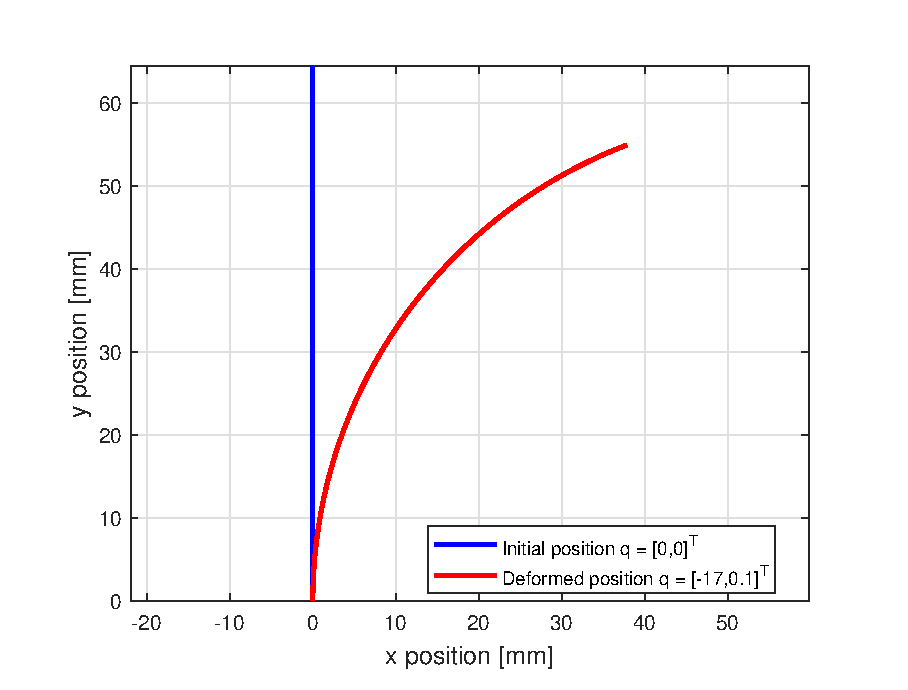
\includegraphics[width = 0.7\textwidth]{Figures/Chapter2/fkin1701.eps}
    \caption{Initial position and deformed position for a first order shape function approximation of the kinematic model.}
    \label{fig1:forward_kinematic}
\end{figure}

Besides a forward kinematic model, a numerical inverse kinematic solver was programmed. This allows to define a position in planar Cartesian coordinates. The algorithm will minimize the distance between the desired end-effector position and reachable end-effector position given an amount of shape functions is in its approximations. It shows the model's flexibility when using multiple shape functions. The algorithm is further detailed in Appendix \ref{app:chap2}. 

For now we have neglected the time dependency of modal coordinate vector $q(t)$. To determine the dynamics of the system it is crucial to consider the time variance of the system to as well. In order to do so, we first consider the velocity kinematics of the system in the next section.


\section{Velocity kinematics}

The velocity kinematics allows us to study velocities along the backbone curve. Similar to the spatial derivative, backbone curve $g(\sigma,t)$ can be differentiated with respect to time. This differentiation results in, 

\begin{equation}
  \Dot{g} = \frac{\partial g}{\partial t} = g \hat{\eta} \hspace{10pt} \text{with} \hspace{10pt}  \hat{\eta} = \begin{pmatrix} \Omega_\times & V \\ 0_3^\top & 0 \end{pmatrix} \in  \mathfrak{se}(2)
    \label{eq2:dgdt}
\end{equation}

which describes the time-twist field in a local frame at $\sigma$. Here, $\Omega_\times \in \mathfrak{so}(2)$ is a skew-symmetric matrix expressing angular velocity, and vector $V = [v_1,v_2]^\top \in \mathbb{R}^2$ contains linear velocities. Therefore, $\hat{\eta} \in \mathfrak{se}(2)$ effectively contains angular and linear velocities among the backbone curve. The skew-symmetric matrix $\Omega_\times$ contains a single angular velocity component $\omega$. All velocities can equivalently be stored in column vector $\eta(\sigma,t) = [\Omega^\top \hspace{5pt} V^\top]^\top \in \mathbb{R}^3$ \cite{Sola2018}.

Using the equality of mixed partial derivatives, at each instant of space and time $\frac{\partial}{\partial t}g' = \frac{\partial}{\partial \sigma}\dot{g}$ holds \cite{Caasenbrood2020}. By using general rules of substitution and actions in Lie space it can be proven that the spatial derivative of the velocity field can be written as,

\begin{equation}
    \eta'= (\text{Ad}_g^{-1})'\text{Ad}_g \eta + \Dot{\xi} \hspace{10pt} \text{with} \hspace{10pt} \text{Ad}_g = \begin{bmatrix} 0_{1 \times 2} & 1 \\ p_\times & R  \end{bmatrix} \in \mathbb{R}^{3\times 3}
    \label{eq2:etadif}
\end{equation}


where $\text{Ad}_g \in \mathbb{R}^{3 \times 3}$ \cite{2DLie} is the adjoint mapping of $g$ \cite{Sola2018}. Here, $p_\times$ is defined as $[p_2 \hspace{4pt} -p_1]^\top$ \cite{2DLie}. The complete derivation is presented in Appendix \ref{app:chap2}. 

An analytic solution to \ref{eq2:etadif} can be found by integrating the equation over spatial domain $[0,\sigma]$. It is given that the actuator is fixed at one end. Therefore the boundary conditions $\eta_0 = 0_{3 \times 1}$ and $g_0 = I_{3\times 3}$ can be imposed. This physically means that at $\sigma = 0$ there is no velocity, strain nor curvature. Integrating over domain $[0,\sigma]$ will give accordingly,

\begin{equation}
  \begin{bmatrix} \eta(\sigma,t)\end{bmatrix}_N = \text{Ad}_{[g]_N^{-1}} \int_0^{\sigma} \text{Ad}_{[g]_N} B_a \Phi(\sigma) d \sigma \dot{q} = [J(\sigma,t)]\dot{q}(t)
    \label{eq2:J}
\end{equation}

here an expression for the geometric Jacobian $J(\sigma,t) \in \mathbb{R}^{3\times 2}$ is obtained \cite{Caasenbrood2020}. This Jacobian maps modal coordinate velocity to linear and angular velocities along the backbone curve. Let us be clear on the dimension of this geometric Jacobian. 
Since we have two active degrees of freedom, that are strain $\epsilon$ in y-direction and curvature strain $\kappa$, our modal coordinate vector $q(t)$ has length two. The geometric Jacobian maps the modal coordinate velocity $\dot{q}(t)$ to velocities in the Euclidean space. The velocity of a point with respect to a reference in 2 dimensional Euclidean space can be described by 3 components. From our fixed reference point at $g(0,t)$, these velocities are one rotational velocity, and two linear velocities in horizontal en vertical direction, respectively. As can be seen, this Jacobian matrix is non-linear with respect to position and time. Besides relating modal coordinate velocity to Cartesian velocity, the Jacobian can be used on position level as,

\begin{equation}
    [r(\sigma,t)] = [J(\sigma,t))]q(t),
\end{equation}

which implies that modal coordinates $q(t)$ can also be mapped to a position vector $r\in \mathbb{R}^3$ in Euclidean space. This position vector contains rotation, horizontal and vertical position as $[\theta \hspace{3pt} x \hspace{3pt} y]^\top$, respectively. Therefore this Jacobian is of valuable use for further system analysis. It can for instance be used in path-planning, as the Jacobian inverse can map Cartesian coordinates to modal coordinates. Furthermore, it can be used in controller design. However, next the Jacobian will be used for deriving the dynamics of the soft robot. 


\section{Dynamic model derivation}


To study the dynamic behaviour of the soft actuator a dynamic model is created. A relatively simple approximation is used to get insight of the basic dynamics of the actuator. The dynamic model will primarily be used for controller design. A relatively simple model is deemed to be sufficient in order to asses general controller performance. To this end, we propose a non-linear mass-spring-damper model. In previous section we obtained an expression for the Jacobian matrix. Here we observed its position an time variance, therefore it is assumed that mass matrix of the system is also non-linear. Furthermore, it is known that the elastomer of which the soft actuator is composed deforms non-linear. Therefore sought after form to describe our soft robot dynamics is,


\begin{equation}
    M(q)\Ddot{q} + D\dot{q} + K(q)q = \nu,
    \label{eq2:simp_model}
\end{equation}


here $M(q) \in \mathbb{R}^{2\times 2}$ is the non-linear mass matrix. Furthermore, $D \in \mathbb{R}^{2\times2}$ is a linear damping matrix and lastly $K(q) \in \mathbb{R}^{2\times 2}$. Force input $\nu \in \mathbb{R}^2$ describes the input moment and force acting on curvature and elongation, respectively. In this section we detail the derivation of each of these matrices. 

To obtain the mass matrix of the system, we use the Euler-Lagrange method as used in \cite{Caasenbrood2020}. This method include

Since we have an expression for modal coordinate velocity, the total kinetic energy of the system is given by,

\begin{equation}
\mathcal{T} - \mathcal{V} = \mathcal{Q} \hspace{10pt} \text{with} \mathcal{Q} = \mathcal{Q}^{nc} + \mathcal{Q}^c,    
\end{equation}




\begin{equation}
    \mathcal{T} = \frac{1}{2}\int_0^{\sigma} \eta(\sigma,t)^\top \mathcal{M} \eta(\sigma,t) d \sigma  = \frac{1}{2}\int_0^{\sigma} (J \dot{q})^\top \mathcal{M} J\dot{q} d \sigma
    \label{eq2:T}
\end{equation}

where $\mathcal{M} \in \mathbb{R}^{6\times6}$ is a diagonal mass tensor. In our modelling approach, the actuator kinematics have been described by a one-dimensional backbone curve. In order to derive the dynamics, mass properties need to be assigned to this curve. Therefore the backbone curve is discretized, and we consider a cross section of the actuator. In determining the mass of the system the following assumption is made. 

\begin{theorem}
Inertial properties of the actuator can be determined by considering an infinitely thin slice in transverse direction, and regarding it as a solid cuboid.
\end{theorem}


Figure (\ref{fig:massapprox}) shows such a discretized cross section. Here the blue marked area is a solid cuboid with height $h$, width $w$, density $\rho$ and slice thickness $d\sigma$. 

\clearpage

\begin{figure}[H]
    \centering
    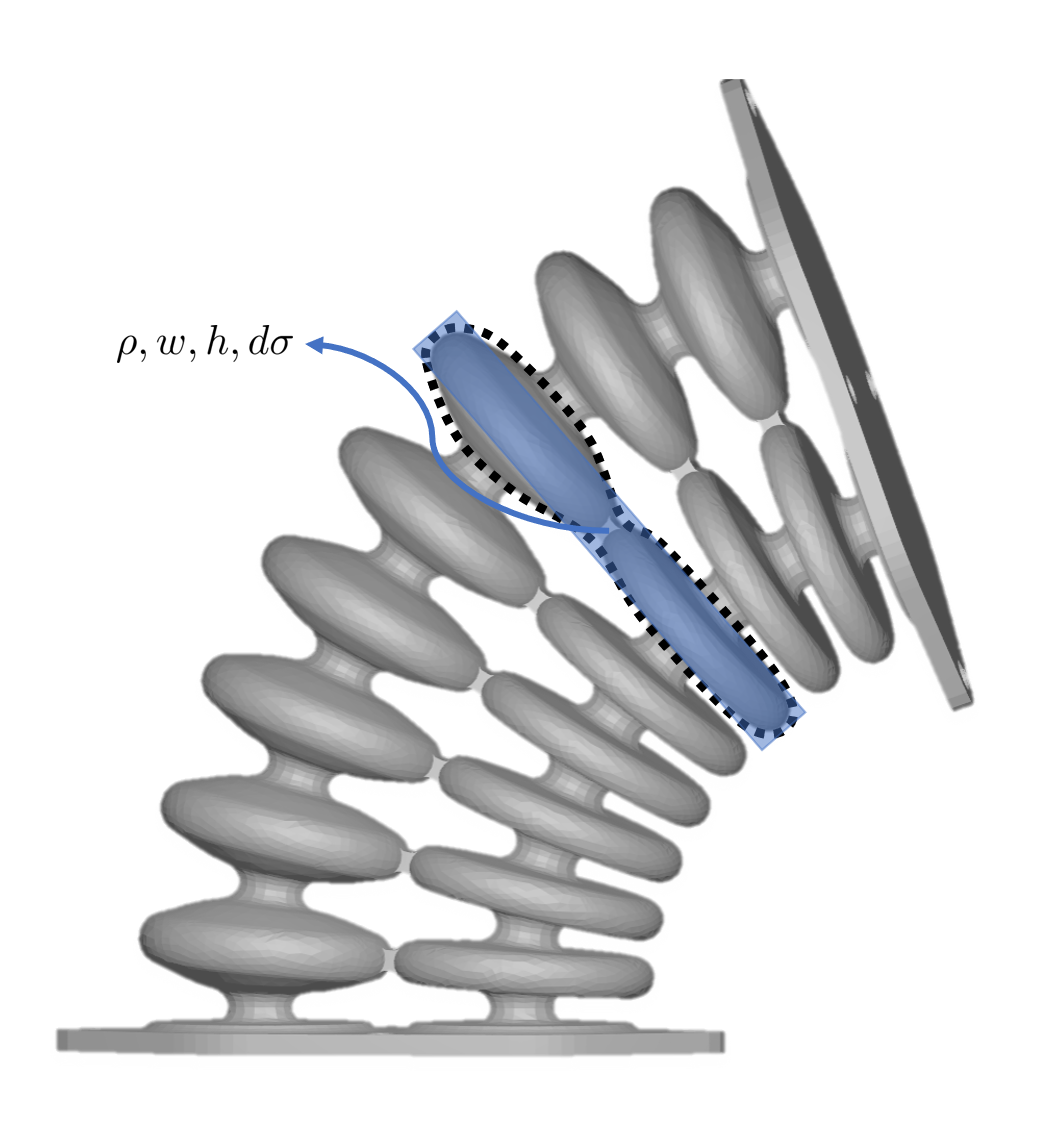
\includegraphics[width = 0.4\textwidth]{Figures/Chapter2/massapprox.png}
    \caption{Inertial properties can be determined by regarding an infinitely thin slice. The cross section is then viewed a solid cuboid.}
    \label{fig:massapprox}
\end{figure}

The mass tensor $\mathcal{M}$ then takes the following form,

\begin{equation}
    \mathcal{M} = \begin{pmatrix} \frac{1}{12}\rho (w^2 + d^2) & 0 & 0 & 0 & 0 & 0 \\
                                  0 & \frac{1}{12}\rho (w^2 + h^2) & 0 & 0 & 0 & 0 \\
                                  0 & 0 & \frac{1}{12}\rho (d^2 + h^2) & 0 & 0 & 0 \\
                                  0 & 0 & 0 & \rho & 0 & 0 \\
                                  0 & 0 & 0 & 0 & \rho & 0 \\
                                  0 & 0 & 0 & 0 & 0 & \rho \end{pmatrix}\hspace{5pt} \text{with} \hspace{5pt} \rho = \frac{m_{tot}}{L_0}
\end{equation} 




where $m_{tot}$ is the total mass of the actuator. The first three entries express mass moments of inertia, related to curvature of the actuator. The last three entries relate to linear velocities of centre of mass of the cuboid. Based on equation (\ref{eq2:T}) the position variant mass matrix can be expressed as, 


\begin{equation}
    M(q) = \int_0^{\sigma} J(\sigma)^\top \mathcal{M}(\sigma)J(\sigma) d \sigma.
\end{equation}

Furthermore damping and stiffness properties are assigned to the actuator. We assume that the polymer of which the actuator is made has linear damping characteristics. An expression for the damping matrix is obtained by,

\begin{equation}
    D = \int_0^\sigma (B_a \Phi(\sigma))^\top  \mathcal{D} (B_a \Phi(\sigma)) d\sigma,
\end{equation}

where $\mathcal{D} \in \mathbb{R}^{6 \times 6}$ is a diagonal damping tensor. For a fact, we know that polymer has non-linear stiffness properties. Therefore stiffness matrix $K$ is position variant, and is therefore given by,

\begin{equation}
    K(q) = \int_0^\sigma (B_a \Phi(\sigma) )^\top \mathcal{K}(q) (B_a \Phi(\sigma))  d\sigma,
\end{equation}

where $\mathcal{K} \in \mathbb{R}^{6 \times 6}$ is a diagonal stiffness tensor. The actuator dynamics that are obtained are then given by,







\section{Actuator dynamics}




\begin{equation}
    p(t) = -\frac{1}{\tau_s} + \frac{R}{\tau_s}V(t)
\end{equation}







%\begin{figure}[H]
%        \centering
%        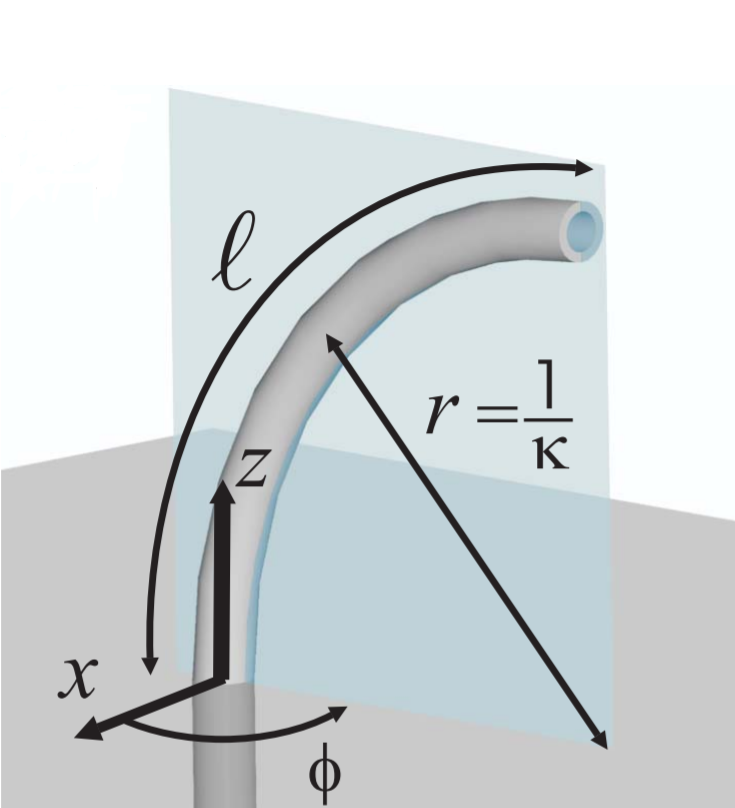
\includegraphics[width=0.85\linewidth]{Figures/Chapter2/ccapproach.png}
%         \caption{Schematic drawing of the constant curvature \cite{ccapproach}.}
%         \label{fig2:ccapproach}
%\end{figure}

